\section{Experiment}

\subsection{Data}
To experiment our algorithm we use the dataset 20Newsgroups \cite{Newsgroups20}.
The 20 Newsgroups data set is a collection of approximately 20,000 Newsgroups 
documents, partitioned evenly across 20 different newsgroups. We use also the 
RCV1 dataset \cite{Lewis:2004:RNB:1005332.1005345}. The RCV1 dataset is a 
collection of over 800,000 text documents. For RCV1 dataset, we use only a 
subset of 10,000 documents from RCV1 such that each document belongs to only 
one of the root classes in the class hierarchy. This was detailed in 
[\cite{Deap-K-Means}].\\
Each document are represented by a vector using term frequency-inverse document 
frequency (TFIDF) representation~\cite{doi:10.1108/eb026526}.
The term frequency-inverse document frequency is a method of weighting depicting 
the significance of each word of a document in relative to a corpus.
\begin{equation}
TF(t, X) = \frac{f_{t, X}}{max_{t' \in C}f_{t', X}} 
\end{equation}
\begin{equation}
IDF(t, C) = log(\frac{N}{|X \in C : t \in X|})
\end{equation}
\begin{equation}
TFIDF(t,X,C) = TF(t, X) . IDF(t, C)   
\end{equation}
For each dataset there is a preprocessing step. We remove stopword and keep only
the 2000 words with the top TFIDF scores. We use also a stemming step 
\cite{journals/mtcl/Lovins68} for dataset 20 Newsgroups. 
\subsection{Generate Constraint}
\subsubsection{Lexical Constraints}
To generate the set of keywords $KW$ we rank each word of each 
document of each class using TFIDF according to algorithm~\ref{algo:gen_kw}.
For our tests, we extract 3 keywords per classes.
\begin{algorithm}
  \SetKwInOut{Input}{input}
  \SetKwInOut{Output}{output}
  \Input{Corpus C, The number of keywords per classes $P$}
  \Output{KW}
  $KW \gets \{\}$\\
  \ForEach{Class $c_i \in C$}{
    $rank_i \gets [0 ... 0]$\\
    \ForEach{Document $X \in c_i$}{
      \ForEach{Word $w \in X$}{
        $rank_{i,w} \gets rank_{i,w} + TFIDF(w,X, C)$\\
      }
    }
  }
  \If{$Discriminating\_ Extraction$}{
    \ForEach{Class $c_i \in C$}{
      ${rank'}_i \gets rank_i - \sum\limits_{\forall c_j, cj \neq c_i}rank_j$\\
    }
    $rank \gets rank'$
  }
  \ForEach{Class $c_i \in C$}{
    $KW \gets KW \cup \{\{w_1, w_2 ... w_P\} : \not\exists (v_1, v_2) | v_1 \not\in 
    \{w_1, w_2 ... w_P\}, v_2 \in \{w_1, w_2 ... w_P\}, rank_{i,v_1} \ge rank_{i,v_2}\}$\\
  }
  \Return{KW}
  \caption{\label{algo:gen_kw}Extract Keywords}
\end{algorithm}
%\subsubsection{Background Knowledge}
%We generate pairwise constraints randomly accordinf to algorithm
%~\ref{algo:gen_pair}
%\begin{algorithm}[!h]
%  \SetKwInOut{Input}{input}
%  \SetKwInOut{Output}{output}
%  \Input{Corpus C, The set of labels L, The number of pair $N_p$}
%  \Output{Must-Link Pair ML, Cannot-Link Pair CL}
%  \For{p = 1 : $N_p$}{
%    \Repeat{$X_i \neq X_j \wedge L_i = L_j$}{
%      Choose randomly ($X_i, X_j$)\\
%    }
%    Insert ($X_i, X_j$) in ML\\
%  }
%  \For{p = 1 : $N_p$}{
%    \Repeat{$X_i \neq X_j \wedge L_i \neq L_j$}{
%      Choose randomly ($X_i, X_j$)\\
%    }
%    Insert ($X_i, X_j$) in ML\\
%  }
%  \Return{ML, CL}
%  \caption{\label{algo:gen_pair}Extract Pair}
%\end{algorithm}
\subsection{Evaluation}
\subsubsection{Baseline Algorithm}
We evaluate our algorithm with $K$-Means and Deep $K$-Means with pretraining 
see in section~\ref{seq:DeepClust}.
\subsubsection{Metric}
To evaluate our algorithm and compare results with reference algorithms we can
use the NMI Metric, Accuracy Metric \cite{NMI_ACC}, and Adjusted
Rand index\cite{ARI}. 
\begin{itemize}
\item NMI is an information-theoretic measure based on the mutual information of the ground-truth classes
and the obtained clusters, normalized using the entropy of each. The NMI Metric is defined as follows
$$NMI(S,C) = \frac{I(S,C)}{[H(S)+H(C)]/2}$$ 
with
$I(S,C) =\sum\limits_k \sum\limits_f\frac{|s_k \cap c_f|}{N}log\frac{N|s_k \cap c_f|}{|s_k| |c_f|}$
and
$H(S) = -\sum\limits_k\frac{|s_k|}{N}log\frac{N|s_k|}{|s_k|}$
\item The Accuracy is the proportion of true results among the total
  number of cases examined. The Accuracy metric is defined as follows :
$$
ACC(S,C) = \frac{1}{N}\sum\limits_k {max}_j|s_k \cap c_j|
$$
\item Let a be the number of pairs of document in C
  that are in the same cluster in the predicted partition and in the
  same cluster in the real partition, and b be the number of pairs of
  document in C that are in different clusters in predicted partition
  and in different cluster in real partition.
  The Adjusted Rand index is defined as follows :
  $$ARI = \frac{a+b}{\binom{N}{2}}$$
\end{itemize}
\subsection{Experimental Setup}
\subsubsection{Autoencoder Architecture}
We use the same architecture used in~\cite{Deap-K-Means}. The encoder is a fully-connected 
multilayer perceptron formed by 3 hidden layers (with dimensions 500, 500, 2000) 
and an embedding layer (with dimension K, the number of cluster). 
The decoder is a mirrored version of the encoder~\ref{fig:autoenc}.
The ReLu activation function is used on layers, except for the third
hidden layer of encoder and decoder part.
 
\subsubsection{Hyperparameters}
For the $\lambda$ hyperparameter we use the value defined in \cite{Deap-K-Means}. 
For the hyperparameter $\alpha_0$, we used Line Search~\cite{SWANN1969S39} strategy for 
$\alpha_0$ optimization. The Line search was done in two steps :
first, we searched on several range with 2 runs. Then we search on the range 
$[10^{-3},5.10^{-3},10^{-2},5.10^{-2},10^{-1}]$ with 5 runs.   
The results of Line Search are reported 
in table~\ref{tab:res}. Hyperparameters $alpha_1$, $alpha_2$ and $\eta$ 
are set to 0, because we focused on the lexical constraints in the experiments. 
\begin{table}[!h]
\centering
%\resizebox{\hsize}{!}{
  \begin{tabular}{| l | l | l | l |}
    \hline
               & 20NEWS Without noise & 20NEWS With noise & RCV1 Without noise 
\\ \hline
    $\lambda$  & $10^{-3}$            & $10^{-2}$         & $10^{-4}$           
\\ \hline
    $\alpha_0$ & $5.10^{-2}$          & $5.10^{-3}$       & $10^{-2}$           
\\ \hline
  \end{tabular}
%}
  \caption{\label{tab2}Best results of Line Search for the optimization of
hyperparameters for each dataset.}
\end{table}
\subsubsection{\label{section:test1}Clustering without Noise}
The purpose of the experiment is to rediscover the different classes of the
dataset with keywords and background knowledge.

\subsubsection{\label{section:test2}Clustering with Noise}
We divide the dataset into two corpus $C_1, C_2$. Each corpus contain
ten classes. We generate keywords \ref{algo:gen_kw} from $C_1$. Then we 
add noise to the corpus
$C_1$. To add noise, we concatenate document from corpus $C_1$ with document
from corpus $C_2$.
\\The purpose of the experiment is to rediscover the different classes of the
corpus $C_1$ with keywords and background knowledge.

\subsection{Results}
\begin{table}[h]
\caption{\label{tab:res}Clustering with only lexical constraints applies to 
different learned latent space to measure the efficiency of lexical constraints
for $K$-Means algorithm. Performance is measured in terms of NMI, Adjusted Rand 
Index and clustering Accuracy, higher is better. Each cell contains the average
and the standard deviation computed over 10 runs. The best result for each 
metric/dataset is bold.}
\centering
%\resizebox{\hsize}{!}{
  \begin{tabular}{|l|l|l|l|}
    \hline
    & ACC          &ARI           & NMI           \\ \hline
    20NEWS without noise   &$36.1 \pm 2.2$&$13.3 \pm 1.7$&$40.9 \pm 1.6$ \\ \hline
    20NEWS with noise      &$33.1 \pm 2.7$&$8.7 \pm 1.3$ &$26.3 \pm 1.6$ \\ \hline
    RCV1 without noise     &$48.8 \pm 6.6$&$18.4 \pm 6.0$&$29.7 \pm 5.8$ \\ \hline
  \end{tabular}
%}
\subcaption*{K-Means}
%\resizebox{\hsize}{!}{
  \begin{tabular}{|l|l|l|l|}
    \hline
    & ACC          &ARI          & NMI          \\ \hline
    20NEWS without noise    & $54.9\pm 1.7$&$37.6\pm 1.1$&$51.6\pm 0.6$ \\ \hline
    20NEWS with noise       & $44.5\pm 2.4$&$23.6\pm 2.4$&$30.2\pm 2.0$ \\ \hline
    RCV1 without noise      &$54.4\pm 4.9$ &$23.9\pm 3.5$&$29.6\pm 3.6$ \\ \hline
  \end{tabular}
%}
\subcaption*{Deep K-Means}
%\resizebox{\hsize}{!}{
  \begin{tabular}{|l|l|l|l|}
    \hline
    & ACC                  &ARI                   & NMI                   \\ \hline
    20NEWS without noise   &$55.7\pm 2.3$  &$39.1\pm 1.1$    &$51.9\pm 0.7$ \\ \hline
    20NEWS with noise      &\boldmath$45\pm 1.8$  &\boldmath$22.8\pm 1.1$&\boldmath$28.9\pm 0.8$ \\ \hline
    RCV1 without noise     &\boldmath$64.6\pm 5.7$&\boldmath$31.0\pm 5.0$&\boldmath$36.7 \pm 4.2$  \\ \hline
  \end{tabular}
%}
\subcaption*{Constrained Deep K-means, Lexical Pretrain}
%\resizebox{\hsize}{!}{
  \begin{tabular}{|l|l|l|l|}
    \hline
    & ACC                  &ARI                   & NMI                   \\ \hline
    20NEWS without noise   &$57.6\pm 2.2$  &$39.8\pm 1.2$    &$52.6\pm 0.6$ \\ \hline
    20NEWS with noise      &\boldmath$44.5\pm 2.5$  &\boldmath$24.0\pm 2.3$&\boldmath$30.5\pm 2.$ \\ \hline
    RCV1 without noise     &$57.4\pm 6.4$&$29.1\pm 4.3$&$34.8 \pm 5.3$  \\ \hline
  \end{tabular}
%}
\subcaption*{Constrained Deep K-means,  Simple Pretrain}
%\resizebox{\hsize}{!}{
  \begin{tabular}{|l|l|l|l|}
    \hline
    & ACC                  &ARI                   & NMI                   \\ \hline
    20NEWS without noise   &$55.7\pm 2.5$  &$39.4\pm 1.1$    &$52.1\pm 0.8$ \\ \hline
    20NEWS with noise      &$44.3\pm 1.8$  &\boldmath$24.4\pm 1$&$30.6\pm 0.8$ \\ \hline
    RCV1 without noise     &$53.3\pm 5.2$&$26.3\pm 5.2$&$32.8 \pm 4.2$  \\ \hline
  \end{tabular}
%}
\subcaption*{Constrained Deep K-means, Lexical Pretrain with adding class $r_0$}
%\resizebox{\hsize}{!}{
  \begin{tabular}{|l|l|l|l|}
    \hline
    & ACC                  &ARI                   & NMI                   \\ \hline
    20NEWS without noise   &\boldmath$58.8\pm 2$  &\boldmath$41.3\pm 1.4$    &\boldmath$53.5\pm 0.8$ \\ \hline
    20NEWS with noise      &$43.7\pm 1.6$  &$24.3\pm 1.3$&\boldmath$30.7\pm 1.2$ \\ \hline
    RCV1 without noise     &$52.2\pm 5.3$&$22.9\pm 4$&$29.4 \pm 3.7$  \\ \hline
  \end{tabular}
%}
\subcaption*{Constrained Deep K-means, Simple Pretrain with adding class $r_0$}
\end{table}

\subsection{Robustness}
We can also test the robustness of our algorithm. To test this, we
can vary the number of key words by classes. In addition we compare
the results of each version of our two methods (simple/lexical pretrain, adding 
class) for each dataset.
We can see results  in 
figures \ref{fig:rcv1}, \ref{fig:20news}, \ref{fig:20news_noise}.
\begin{figure}[!h]
\begin{subfigure}[b]{\textwidth}
\begin{minipage}{0.5\linewidth}
\centering
  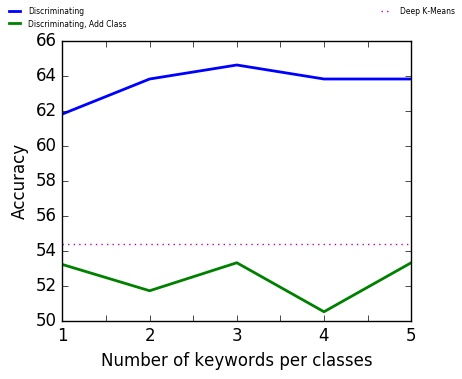
\includegraphics[scale=0.49]{parts/res/dat_file/acc/RCV1.jpg}     
\subcaption{Lexical Pretrain}  
\end{minipage}
  \begin{minipage}{0.5\linewidth}
\centering
   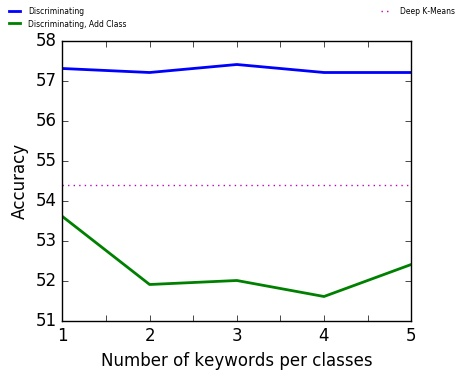
\includegraphics[scale=0.49]{parts/res/dat_file/acc/RCV1_simple.jpg}     
   \subcaption{Simple Pretrain}
\end{minipage}
\end{subfigure}
\begin{subfigure}[b]{\textwidth}
\begin{minipage}{0.5\linewidth}
\centering
  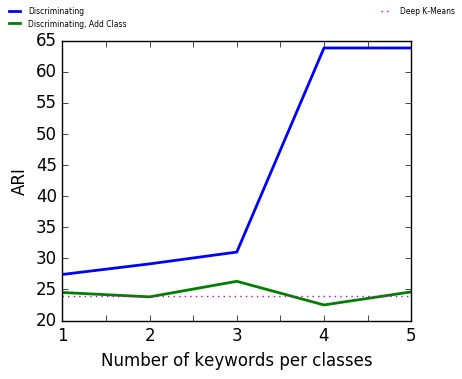
\includegraphics[scale=0.49]{parts/res/dat_file/ari/RCV1.jpg}     
\subcaption{Lexical Pretrain}  
\end{minipage}
  \begin{minipage}{0.5\linewidth}
\centering
   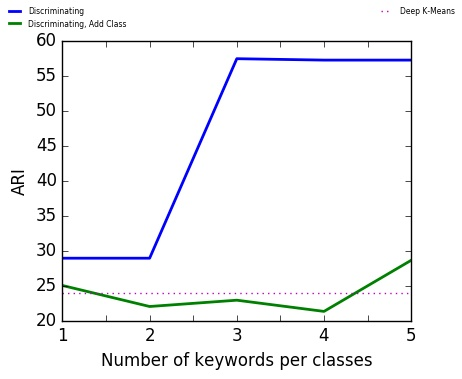
\includegraphics[scale=0.49]{parts/res/dat_file/ari/RCV1_simple.jpg}     
   \subcaption{Simple Pretrain}
\end{minipage}
\end{subfigure}
\begin{subfigure}[b]{\textwidth}
\begin{minipage}{0.5\linewidth}
\centering
  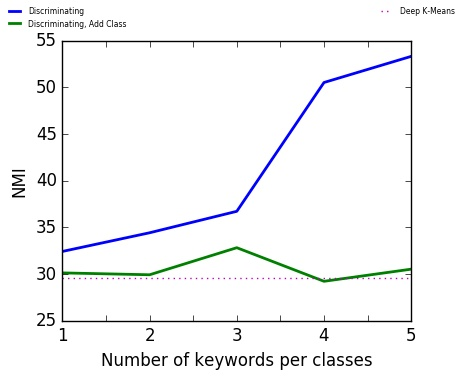
\includegraphics[scale=0.49]{parts/res/dat_file/nmi/RCV1.jpg}     
\subcaption{Lexical Pretrain}  
\end{minipage}
  \begin{minipage}{0.5\linewidth}
\centering
   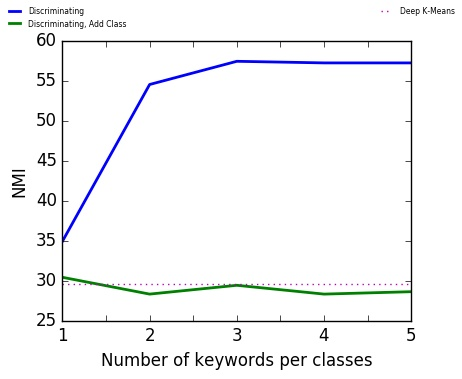
\includegraphics[scale=0.49]{parts/res/dat_file/nmi/RCV1_simple.jpg}     
   \subcaption{Simple Pretrain}
\end{minipage}
\end{subfigure}
\caption{\label{fig:rcv1}Results for RCV1 dataset}
\end{figure}



\begin{figure}[!h]
\begin{subfigure}[b]{\textwidth}
\begin{minipage}{0.5\linewidth}
\centering
  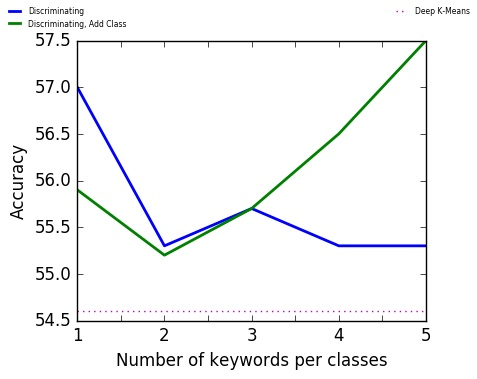
\includegraphics[scale=0.49]{parts/res/dat_file/acc/20NEWS.jpg}     
\subcaption{Lexical Pretrain}  
\end{minipage}
  \begin{minipage}{0.5\linewidth}
\centering
   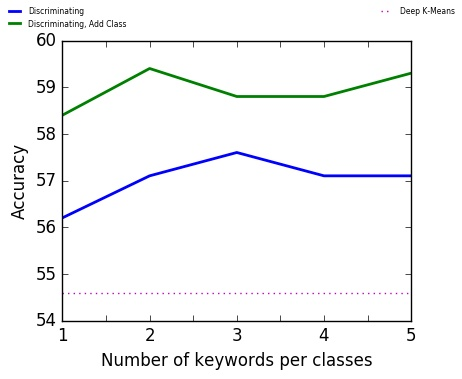
\includegraphics[scale=0.49]{parts/res/dat_file/acc/20NEWS_simple.jpg}     
   \subcaption{Simple Pretrain}
\end{minipage}
\end{subfigure}
\begin{subfigure}[b]{\textwidth}
\begin{minipage}{0.5\linewidth}
\centering
  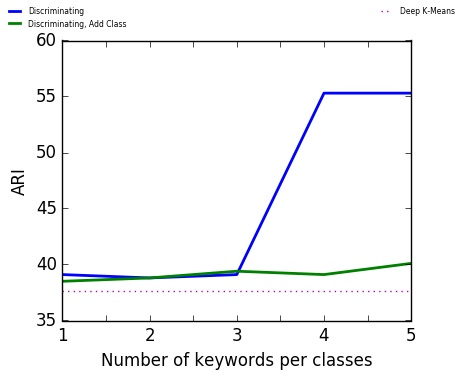
\includegraphics[scale=0.49]{parts/res/dat_file/ari/20NEWS.jpg}     
\subcaption{Lexical Pretrain}  
\end{minipage}
  \begin{minipage}{0.5\linewidth}
\centering
   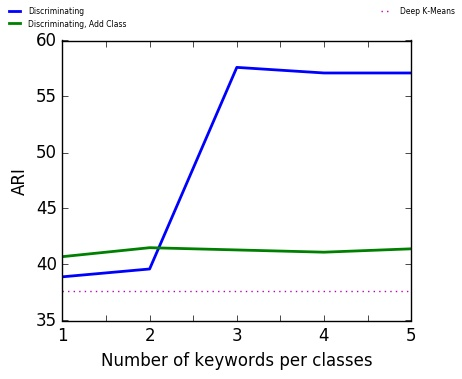
\includegraphics[scale=0.49]{parts/res/dat_file/ari/20NEWS_simple.jpg}     
   \subcaption{Simple Pretrain}
\end{minipage}
\end{subfigure}
\begin{subfigure}[b]{\textwidth}
\begin{minipage}{0.5\linewidth}
\centering
  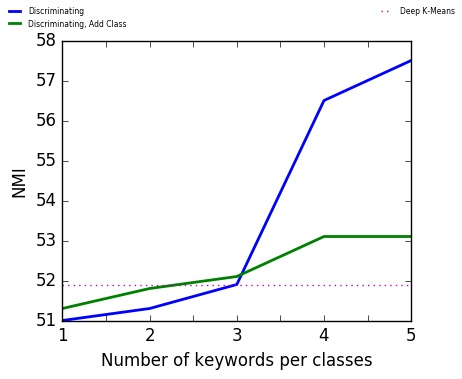
\includegraphics[scale=0.49]{parts/res/dat_file/nmi/20NEWS.jpg}     
\subcaption{Lexical Pretrain}  
\end{minipage}
  \begin{minipage}{0.5\linewidth}
\centering
   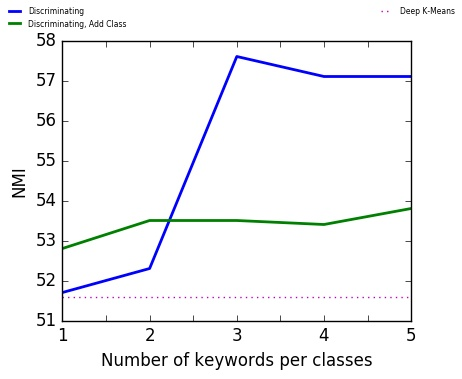
\includegraphics[scale=0.49]{parts/res/dat_file/nmi/20NEWS_simple.jpg}     
   \subcaption{Simple Pretrain}
\end{minipage}
\end{subfigure}\caption{\label{fig:20news}Results for 20 newsgroups dataset without noise}
\end{figure}



\begin{figure}[!h]
\begin{subfigure}[b]{\textwidth}
\begin{minipage}{0.5\linewidth}
\centering
  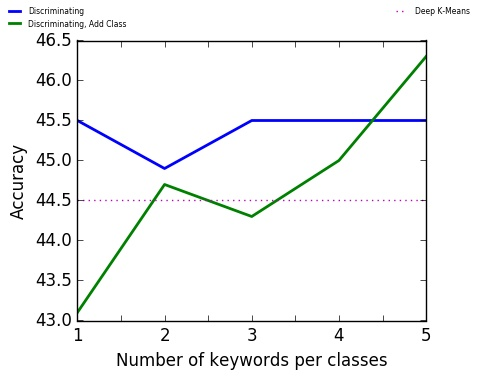
\includegraphics[scale=0.49]{parts/res/dat_file/acc/20NEWS_noisy.jpg}     
\subcaption{Lexical Pretrain}  
\end{minipage}
  \begin{minipage}{0.5\linewidth}
\centering
   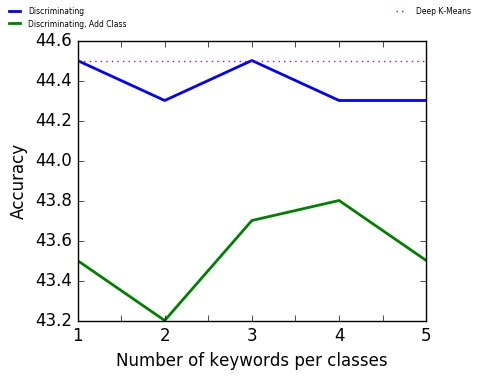
\includegraphics[scale=0.49]{parts/res/dat_file/acc/20NEWS_noisy_simple.jpg}     
   \subcaption{Simple Pretrain}
\end{minipage}
\end{subfigure}
\begin{subfigure}[b]{\textwidth}
\begin{minipage}{0.5\linewidth}
\centering
  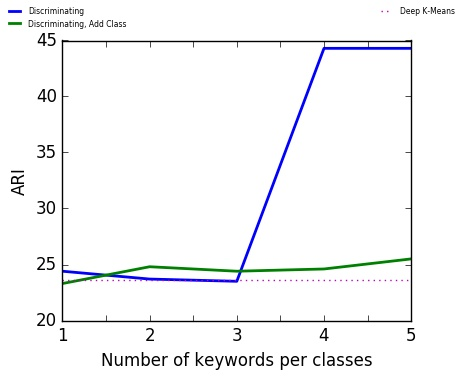
\includegraphics[scale=0.49]{parts/res/dat_file/ari/20NEWS_noisy.jpg}     
\subcaption{Lexical Pretrain}  
\end{minipage}
  \begin{minipage}{0.5\linewidth}
\centering
   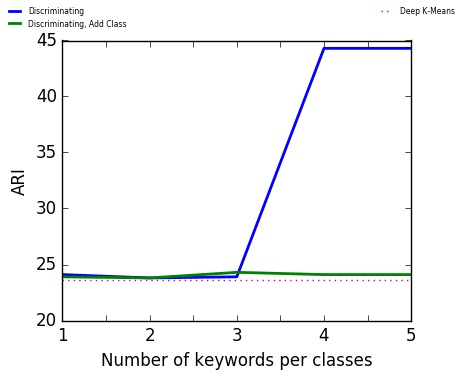
\includegraphics[scale=0.49]{parts/res/dat_file/ari/20NEWS_noisy_simple.jpg}     
   \subcaption{Simple Pretrain}
\end{minipage}
\end{subfigure}
\begin{subfigure}[b]{\textwidth}
\begin{minipage}{0.5\linewidth}
\centering
  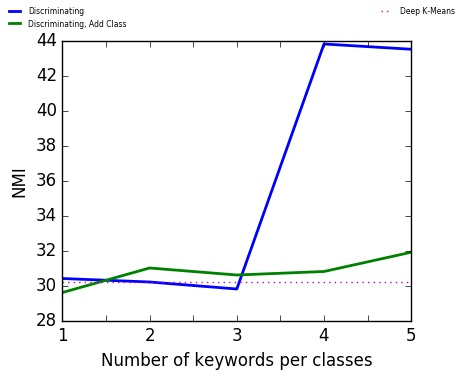
\includegraphics[scale=0.49]{parts/res/dat_file/nmi/20NEWS_noisy.jpg}     
\subcaption{Lexical Pretrain}  
\end{minipage}
  \begin{minipage}{0.5\linewidth}
\centering
   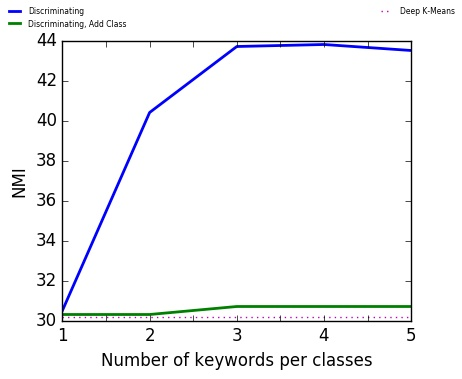
\includegraphics[scale=0.49]{parts/res/dat_file/nmi/20NEWS_noisy_simple.jpg}     
   \subcaption{Simple Pretrain}
\end{minipage}
\end{subfigure}\caption{\label{fig:20news_noise}Results for 20 newsgroups dataset with noise}
\end{figure}

\subsection{Previous Results}
In this, we can see results when there are not stemming step in 
the preprocessing step. We can see results in figure \ref{fig:previous} and in table \ref{tab:res_prev}.
\begin{table}[h]
\caption{\label{tab:res_prev}Previous results for $K$-Means and Deep $K$-Means}
\centering
%\resizebox{\hsize}{!}{
  \begin{tabular}{|l|l|l|l|}
    \hline
    & ACC          &ARI           & NMI           \\ \hline
    20NEWS without noise   &$33.3 \pm 1.9$&$11.6 \pm 1.2$&$36.3 \pm 1.3$ \\ \hline
    20NEWS with noise      &$34.5 \pm 1.5$&$8.7 \pm 0.8$ &$26.3 \pm 2.1$ \\ \hline
    RCV1 without noise     &$48.8 \pm 6.6$&$18.4 \pm 6.0$&$29.7 \pm 5.8$ \\ \hline
  \end{tabular}
%}
\subcaption*{K-Means}
%\resizebox{\hsize}{!}{
  \begin{tabular}{|l|l|l|l|}
    \hline
    & ACC          &ARI          & NMI          \\ \hline
    20NEWS without noise    & $51.7\pm 2.4$&$34.4\pm 1.1$&$47.4\pm 0.8$ \\ \hline
    20NEWS with noise       & $43.4\pm 1.6$&$21.6\pm 0.9$&$28.5\pm 1.0$ \\ \hline
    RCV1 without noise      &$54.4\pm 4.9$ &$23.9\pm 3.5$&$29.6\pm 3.6$ \\ \hline
  \end{tabular}
%}
\subcaption*{Deep K-Means}
\end{table}
\begin{figure}[!h]
  \begin{minipage}{0.5\linewidth}
    \centering
    \includegraphics[scale=0.6]{parts/res/dat_file/20NEWS_old.png}     
    \subcaption{20 Newsgroups without noise}  
  \end{minipage}
  \begin{minipage}{0.5\linewidth}
    \centering
    \includegraphics[scale=0.6]{parts/res/dat_file/RCV1_old.png}     
    \subcaption{RCV1 without noise}
  \end{minipage}
  \caption{\label{fig:previous}Previous results}
\end{figure}
\subsection{Add Class new version}
In this part, we test another way to integrate adding class.
